\documentclass{standalone}
\usepackage{tikz}
\usetikzlibrary{patterns, positioning}

\begin{document}
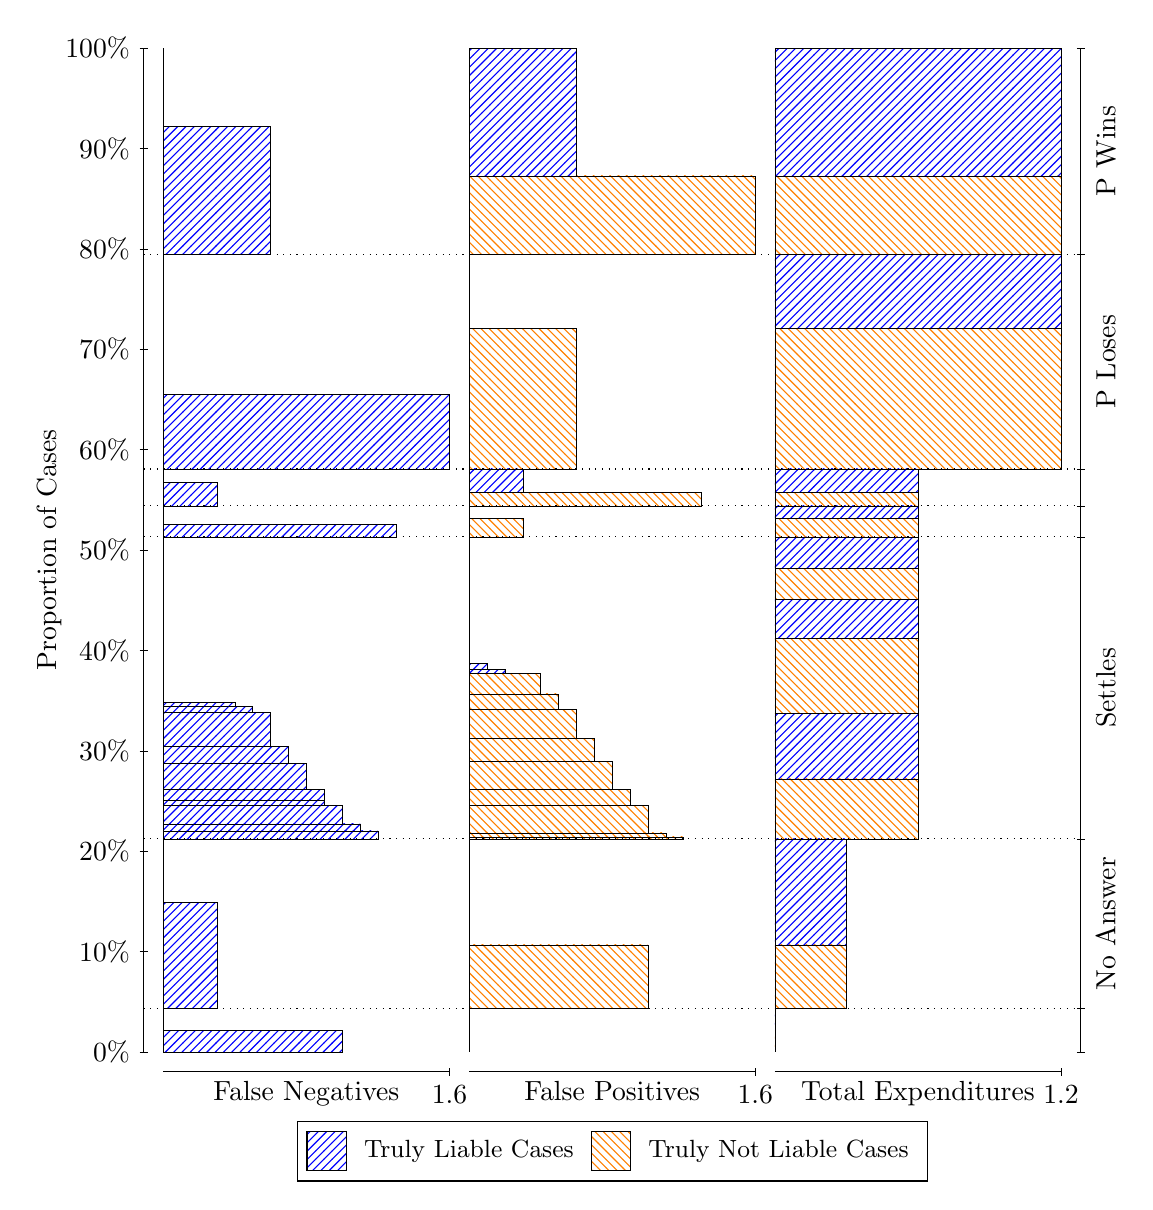
\begin{tikzpicture}
\draw[black, very thin] (1.5,1.75) -- (1.5,14.5);
\node[rotate=90, anchor=center] at (0.3, 8.125) {Proportion of Cases};
\draw[black, very thin] (1.45,1.75) -- (1.55,1.75);
\node[anchor=east] at (1.45, 1.75) {0\%};
\draw[black, very thin] (1.45,3.025) -- (1.55,3.025);
\node[anchor=east] at (1.45, 3.025) {10\%};
\draw[black, very thin] (1.45,4.3) -- (1.55,4.3);
\node[anchor=east] at (1.45, 4.3) {20\%};
\draw[black, very thin] (1.45,5.575) -- (1.55,5.575);
\node[anchor=east] at (1.45, 5.575) {30\%};
\draw[black, very thin] (1.45,6.85) -- (1.55,6.85);
\node[anchor=east] at (1.45, 6.85) {40\%};
\draw[black, very thin] (1.45,8.125) -- (1.55,8.125);
\node[anchor=east] at (1.45, 8.125) {50\%};
\draw[black, very thin] (1.45,9.4) -- (1.55,9.4);
\node[anchor=east] at (1.45, 9.4) {60\%};
\draw[black, very thin] (1.45,10.675) -- (1.55,10.675);
\node[anchor=east] at (1.45, 10.675) {70\%};
\draw[black, very thin] (1.45,11.95) -- (1.55,11.95);
\node[anchor=east] at (1.45, 11.95) {80\%};
\draw[black, very thin] (1.45,13.225) -- (1.55,13.225);
\node[anchor=east] at (1.45, 13.225) {90\%};
\draw[black, very thin] (1.45,14.5) -- (1.55,14.5);
\node[anchor=east] at (1.45, 14.5) {100\%};

\draw[black, very thin] (13.4,1.75) -- (13.4,14.5);
\draw[black, very thin] (13.35,1.75) -- (13.45,1.75);
\node[anchor=west] at (13.35, 1.75) {};
\draw[black, very thin] (13.35,2.3031) -- (13.45,2.3031);
\node[anchor=west] at (13.35, 2.3031) {};
\draw[black, very thin] (13.35,4.4559) -- (13.45,4.4559);
\node[anchor=west] at (13.35, 4.4559) {};
\draw[black, very thin] (13.35,8.2912) -- (13.45,8.2912);
\node[anchor=west] at (13.35, 8.2912) {};
\draw[black, very thin] (13.35,8.6858) -- (13.45,8.6858);
\node[anchor=west] at (13.35, 8.6858) {};
\draw[black, very thin] (13.35,9.1544) -- (13.45,9.1544);
\node[anchor=west] at (13.35, 9.1544) {};
\draw[black, very thin] (13.35,11.881) -- (13.45,11.881);
\node[anchor=west] at (13.35, 11.881) {};
\draw[black, very thin] (13.35,14.5) -- (13.45,14.5);
\node[anchor=west] at (13.35, 14.5) {};

\draw[black, very thin, pattern color=blue, pattern=north east lines] (1.75,1.75) rectangle (4.0208,2.0269);
\draw[black, very thin, pattern color=orange, pattern=north west lines] (1.75,2.0269) rectangle (1.75,2.3031);
\draw[black, very thin, pattern color=blue, pattern=north east lines] (1.75,2.3031) rectangle (2.4312,3.6491);
\draw[black, very thin, pattern color=orange, pattern=north west lines] (1.75,3.6491) rectangle (1.75,4.4559);
\draw[black, very thin, pattern color=blue, pattern=north east lines] (1.75,4.4559) rectangle (4.475,4.5589);
\draw[black, very thin, pattern color=blue, pattern=north east lines] (1.75,4.5589) rectangle (4.2479,4.6458);
\draw[black, very thin, pattern color=blue, pattern=north east lines] (1.75,4.6458) rectangle (4.0208,4.8772);
\draw[black, very thin, pattern color=blue, pattern=north east lines] (1.75,4.8772) rectangle (3.7937,4.9508);
\draw[black, very thin, pattern color=blue, pattern=north east lines] (1.75,4.9508) rectangle (3.7937,5.0807);
\draw[black, very thin, pattern color=blue, pattern=north east lines] (1.75,5.0807) rectangle (3.5667,5.4118);
\draw[black, very thin, pattern color=blue, pattern=north east lines] (1.75,5.4118) rectangle (3.3396,5.6329);
\draw[black, very thin, pattern color=blue, pattern=north east lines] (1.75,5.6329) rectangle (3.1125,6.0579);
\draw[black, very thin, pattern color=blue, pattern=north east lines] (1.75,6.0579) rectangle (2.8854,6.1374);
\draw[black, very thin, pattern color=blue, pattern=north east lines] (1.75,6.1374) rectangle (2.6583,6.1902);
\draw[black, very thin, pattern color=orange, pattern=north west lines] (1.75,6.1902) rectangle (1.75,8.2912);
\draw[black, very thin, pattern color=blue, pattern=north east lines] (1.75,8.2912) rectangle (4.7021,8.4461);
\draw[black, very thin, pattern color=orange, pattern=north west lines] (1.75,8.4461) rectangle (1.75,8.6858);
\draw[black, very thin, pattern color=blue, pattern=north east lines] (1.75,8.6858) rectangle (2.4312,8.9813);
\draw[black, very thin, pattern color=orange, pattern=north west lines] (1.75,8.9813) rectangle (1.75,9.1544);
\draw[black, very thin, pattern color=blue, pattern=north east lines] (1.75,9.1544) rectangle (5.3833,10.098);
\draw[black, very thin, pattern color=orange, pattern=north west lines] (1.75,10.098) rectangle (1.75,11.881);
\draw[black, very thin, pattern color=blue, pattern=north east lines] (1.75,11.881) rectangle (3.1125,13.505);
\draw[black, very thin, pattern color=orange, pattern=north west lines] (1.75,13.505) rectangle (1.75,14.5);
\draw[black, very thin, pattern color=orange, pattern=north west lines] (5.6333,1.75) rectangle (5.6333,2.0261);
\draw[black, very thin, pattern color=blue, pattern=north east lines] (5.6333,2.0261) rectangle (5.6333,2.3031);
\draw[black, very thin, pattern color=orange, pattern=north west lines] (5.6333,2.3031) rectangle (7.9042,3.1099);
\draw[black, very thin, pattern color=blue, pattern=north east lines] (5.6333,3.1099) rectangle (5.6333,4.4559);
\draw[black, very thin, pattern color=orange, pattern=north west lines] (5.6333,4.4559) rectangle (8.3583,4.4811);
\draw[black, very thin, pattern color=orange, pattern=north west lines] (5.6333,4.4811) rectangle (8.1313,4.5325);
\draw[black, very thin, pattern color=orange, pattern=north west lines] (5.6333,4.5325) rectangle (7.9042,4.8847);
\draw[black, very thin, pattern color=orange, pattern=north west lines] (5.6333,4.8847) rectangle (7.6771,5.08);
\draw[black, very thin, pattern color=orange, pattern=north west lines] (5.6333,5.08) rectangle (7.45,5.4375);
\draw[black, very thin, pattern color=orange, pattern=north west lines] (5.6333,5.4375) rectangle (7.2229,5.7324);
\draw[black, very thin, pattern color=orange, pattern=north west lines] (5.6333,5.7324) rectangle (6.9958,6.1044);
\draw[black, very thin, pattern color=orange, pattern=north west lines] (5.6333,6.1044) rectangle (6.7687,6.2964);
\draw[black, very thin, pattern color=orange, pattern=north west lines] (5.6333,6.2964) rectangle (6.5417,6.557);
\draw[black, very thin, pattern color=blue, pattern=north east lines] (5.6333,6.557) rectangle (6.0875,6.6097);
\draw[black, very thin, pattern color=blue, pattern=north east lines] (5.6333,6.6097) rectangle (5.8604,6.6892);
\draw[black, very thin, pattern color=blue, pattern=north east lines] (5.6333,6.6892) rectangle (5.6333,8.2912);
\draw[black, very thin, pattern color=orange, pattern=north west lines] (5.6333,8.2912) rectangle (6.3146,8.5308);
\draw[black, very thin, pattern color=blue, pattern=north east lines] (5.6333,8.5308) rectangle (5.6333,8.6858);
\draw[black, very thin, pattern color=orange, pattern=north west lines] (5.6333,8.6858) rectangle (8.5854,8.8588);
\draw[black, very thin, pattern color=blue, pattern=north east lines] (5.6333,8.8588) rectangle (6.3146,9.1544);
\draw[black, very thin, pattern color=orange, pattern=north west lines] (5.6333,9.1544) rectangle (6.9958,10.938);
\draw[black, very thin, pattern color=blue, pattern=north east lines] (5.6333,10.938) rectangle (5.6333,11.881);
\draw[black, very thin, pattern color=orange, pattern=north west lines] (5.6333,11.881) rectangle (9.2667,12.876);
\draw[black, very thin, pattern color=blue, pattern=north east lines] (5.6333,12.876) rectangle (6.9958,14.5);
\draw[black, very thin, pattern color=orange, pattern=north west lines] (9.5167,1.75) rectangle (9.5167,2.0261);
\draw[black, very thin, pattern color=blue, pattern=north east lines] (9.5167,2.0261) rectangle (9.5167,2.3031);
\draw[black, very thin, pattern color=orange, pattern=north west lines] (9.5167,2.3031) rectangle (10.425,3.1099);
\draw[black, very thin, pattern color=blue, pattern=north east lines] (9.5167,3.1099) rectangle (10.425,4.4559);
\draw[black, very thin, pattern color=orange, pattern=north west lines] (9.5167,4.4559) rectangle (11.333,5.217);
\draw[black, very thin, pattern color=blue, pattern=north east lines] (9.5167,5.217) rectangle (11.333,6.0526);
\draw[black, very thin, pattern color=orange, pattern=north west lines] (9.5167,6.0526) rectangle (11.333,7.0035);
\draw[black, very thin, pattern color=blue, pattern=north east lines] (9.5167,7.0035) rectangle (11.333,7.4985);
\draw[black, very thin, pattern color=orange, pattern=north west lines] (9.5167,7.4985) rectangle (11.333,7.8875);
\draw[black, very thin, pattern color=blue, pattern=north east lines] (9.5167,7.8875) rectangle (11.333,8.2912);
\draw[black, very thin, pattern color=orange, pattern=north west lines] (9.5167,8.2912) rectangle (11.333,8.5308);
\draw[black, very thin, pattern color=blue, pattern=north east lines] (9.5167,8.5308) rectangle (11.333,8.6858);
\draw[black, very thin, pattern color=orange, pattern=north west lines] (9.5167,8.6858) rectangle (11.333,8.8588);
\draw[black, very thin, pattern color=blue, pattern=north east lines] (9.5167,8.8588) rectangle (11.333,9.1544);
\draw[black, very thin, pattern color=orange, pattern=north west lines] (9.5167,9.1544) rectangle (13.15,10.938);
\draw[black, very thin, pattern color=blue, pattern=north east lines] (9.5167,10.938) rectangle (13.15,11.881);
\draw[black, very thin, pattern color=orange, pattern=north west lines] (9.5167,11.881) rectangle (13.15,12.876);
\draw[black, very thin, pattern color=blue, pattern=north east lines] (9.5167,12.876) rectangle (13.15,14.5);
\draw[black, dotted] (1.5,2.3031) -- (13.4,2.3031);
\draw[black, dotted] (1.5,4.4559) -- (13.4,4.4559);
\draw[black, dotted] (1.5,8.2912) -- (13.4,8.2912);
\draw[black, dotted] (1.5,8.6858) -- (13.4,8.6858);
\draw[black, dotted] (1.5,9.1544) -- (13.4,9.1544);
\draw[black, dotted] (1.5,11.881) -- (13.4,11.881);
\draw[black, very thin] (1.75,1.5) -- (5.3833,1.5);
\node[anchor=north] at (3.5667, 1.5) {False Negatives};
\draw[black, very thin] (5.3833,1.45) -- (5.3833,1.55);
\node[anchor=north] at (5.3833, 1.45) {1.6};

\draw[black, very thin] (5.6333,1.5) -- (9.2667,1.5);
\node[anchor=north] at (7.45, 1.5) {False Positives};
\draw[black, very thin] (9.2667,1.45) -- (9.2667,1.55);
\node[anchor=north] at (9.2667, 1.45) {1.6};

\draw[black, very thin] (9.5167,1.5) -- (13.15,1.5);
\node[anchor=north] at (11.333, 1.5) {Total Expenditures};
\draw[black, very thin] (13.15,1.45) -- (13.15,1.55);
\node[anchor=north] at (13.15, 1.45) {1.2};


\node[black, centered, rotate=90] at (13.72, 3.3795) {No Answer};
\node[black, centered, rotate=90] at (13.72, 6.3736) {Settles};


\node[black, centered, rotate=90] at (13.72, 10.518) {P Loses};
\node[black, centered, rotate=90] at (13.72, 13.191) {P Wins};

\draw (7.449999999999999,1.5) node[draw=none] (baseCoordinate) {};
\begin{scope}[align=center]
        \matrix[scale=0.5, draw=black, below=0.5cm of baseCoordinate, nodes={draw}, column sep=0.1cm]{
            \node[rectangle, draw, minimum width=0.5cm, minimum height=0.5cm, pattern=north east lines, pattern color=blue] {}; &
            \node[draw=none, font=\small] (B) {Truly Liable Cases}; &
            \node[rectangle, draw, minimum width=0.5cm, minimum height=0.5cm, pattern=north west lines, pattern color=orange] {}; &
            \node[draw=none, font=\small] (B) {Truly Not Liable Cases}; \\
            };
\end{scope}

\end{tikzpicture}
\end{document}